% 组会分享：PRB 97, 205409 (2018) 导读
% 编译：cd presentation1 && xelatex presentation1.tex（跑两遍）
\documentclass[aspectratio=169,11pt]{ctexbeamer}

\usepackage{amsmath,amssymb,bm}
\usepackage{graphicx}
\usepackage{booktabs}
\usepackage{xcolor}

\graphicspath{{../figs/}{../../img/TB/}{../../img/TB-reconnected/}{../../img/GW/}{../../doc/fig/}}
\graphicspath{
  {../figs/}
  {../../}
  {../../doc/fig/}
}

\usefonttheme{professionalfonts}
\setbeamertemplate{navigation symbols}{}
\setbeamertemplate{footline}[frame number]
\setbeamertemplate{itemize items}[triangle]
\setbeamerfont{frametitle}{size=\large,series=\bfseries}

\newcommand{\eps}{\varepsilon}
\newcommand{\kk}{\mathbf{k}}
\newcommand{\qq}{\mathbf{q}}
\newcommand{\kq}{\mathbf{k}'}

\definecolor{accent}{HTML}{2E6F9E} %#2E6F9E
\setbeamercolor{frametitle}{fg=accent}
\setbeamercolor{title}{fg=accent}
\setbeamercolor{structure}{fg=accent}

\title{组会分享}
% \subtitle{\texorpdfstring{第一部分：三能带模型的 GW 重拟合\qquad 第二部分：文献导读}{第一部分：三能带模型的 GW 重拟合；第二部分：文献导读}}
% \subtitle{文献导读：Phys. Rev. B \textbf{97}, 205409 (2018)}
\author{Neo Wang}
\date{2026 年 11 月 15 日}

\begin{document}
\begin{frame}[plain]
  \titlepage
\end{frame}

%---------------------------------------------------------------------
\begin{frame}[plain]
  \centering
  {\color{accent}\Huge\bfseries 第一部分}\\[7mm]
  {\Large 三能带模型的 GW 重拟合}\\[4mm]
  {\small 承接上一阶段的 NN / NNN / TNN 建模}
\end{frame}

%---------------------------------------------------------------------
\begin{frame}{模型：从上一阶段接过来}
  \begin{columns}[T]
    \begin{column}{0.54\textwidth}
      \begin{itemize}
        \item 基组取 Mo 的三个 $d$ 轨道 $d_{z^2}$、$d_{xy}$、$d_{x^2-y^2}$，计入自旋后为 6 维。
        \item 由 $D_{3h}$ 对称性，跳跃矩阵的独立参数压到 19 个：
              原位能 2 个、最近邻 6 个、次近邻 5 个、第三近邻 6 个。
        \item 自旋轨道耦合取 $H_{\mathrm{SOC}}=\lambda S_z\otimes L_z$，$\lambda=0.073\,\mathrm{eV}$。
        \item 上一阶段的参数取自文献，对应的是 DFT 层面的能带。
      \end{itemize}
    \end{column}
    \begin{column}{0.44\textwidth}
      \centering
      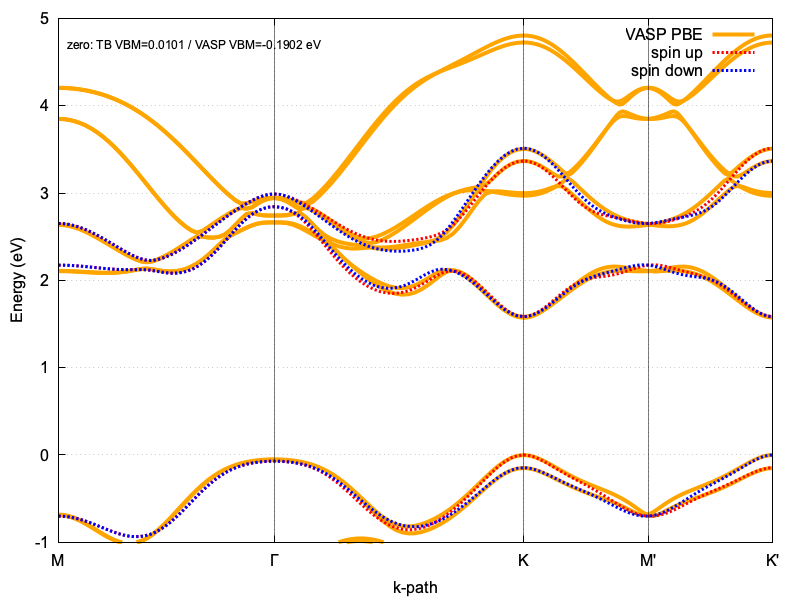
\includegraphics[height=0.50\textheight,keepaspectratio]{img/TB/NN-NNN-TNN-SOC-SPIN.png}\\
      \scriptsize 上一阶段的能带（NN+NNN+TNN，含 SOC 与自旋）
    \end{column}
  \end{columns}
\end{frame}

%---------------------------------------------------------------------
\begin{frame}{这个阶段的目标}
  \begin{columns}[T]
    \begin{column}{0.43\textwidth}
      \vspace{11mm}
      把 19 个参数重新拟合到 GW 能带，模型结构不变。
      \vspace{4mm}
      \begin{itemize}
        \item $E_M \approx E_{\mathrm{gap}} - E_b$\\
              单粒子起点必须是准粒子能带。
        \item 文献参数对应的是 DFT 层面的能带，带隙比 GW 准粒子带隙小。
      \end{itemize}
    \end{column}
    \begin{column}{0.55\textwidth}
      \centering
      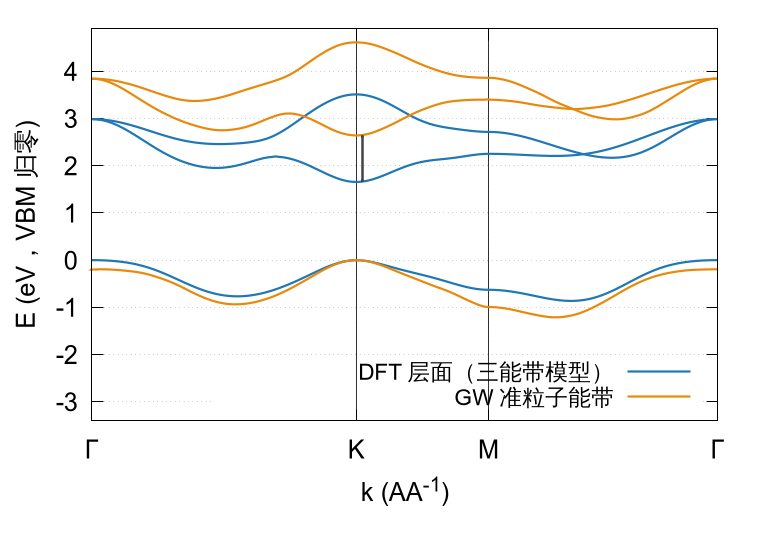
\includegraphics[width=\linewidth]{dft_vs_gw.png}\\
      \scriptsize 同一条 $\Gamma$--K--M--$\Gamma$ 路径上的两套能带：蓝线是文献参数的三能带模型
      （拟合 PBE 能带），橙线是 GW 能带。$K$ 点带隙相差 $0.98\,\mathrm{eV}$。
    \end{column}
  \end{columns}
\end{frame}

%---------------------------------------------------------------------
\begin{frame}{GW 参考能带的身份问题}
  \begin{columns}[T]
    \begin{column}{0.50\textwidth}
      \begin{itemize}
        \item Wannier90 在每个 $k$ 点按能量排序输出，两条带交叉之后序号互换。
        \item 直接连线，交叉处会出现折角。
      \end{itemize}
      \vspace{4mm}
      为了解决这个问题，我实现了如下算法
      \begin{itemize}
        \item 最小曲率拼接：\\
              以 $K$ 点为锚点向两侧逐点走，用前两步线性外推预测位置，
              在全部排列中取 $\sum(\text{位置}-\text{预测})^2$ 最小者。
        \item 但是这套算法在处理自旋导致的能带劈裂时，其在劈裂的能带简并的位置会失效
      \end{itemize}
    \end{column}
    \begin{column}{0.48\textwidth}
      \centering
      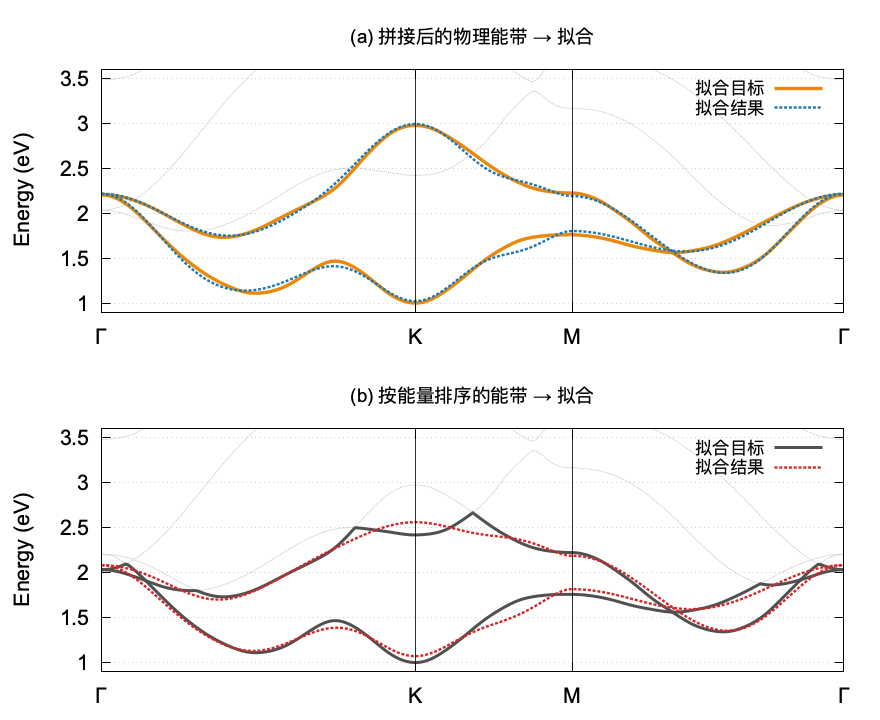
\includegraphics[width=\linewidth]{fig_stitch.png}\\
      \scriptsize (a)拼接后的物理能带当拟合目标；\\
                  (b)不拼接直接拟合；
    \end{column}
  \end{columns}
\end{frame}

%---------------------------------------------------------------------
\begin{frame}{拟合：配对、损失函数、优化}
  \begin{columns}[T]
    \begin{column}{0.52\textwidth}
      \begin{itemize}
        \item 导带配对：模型带 2 对物理带 1，模型带 3 对物理带 3，中间的物理带 2 跳过。
        \item 损失函数取三条带在 285 个 $k$ 点上的均匀加权平方和
              $\mathcal{L}=\sum_{n,\mathbf k}\left[E_{\mathrm{TB}}-E_{\mathrm{GW}}\right]^2$。
        \item 优化用逐参数扫描配步长减半，不依赖梯度；71 轮后最大步长降到 $8\times10^{-7}$。
        \item 初值取文献参数整体平移 $-0.987\,\mathrm{eV}$ 之后出发。
      \end{itemize}
    \end{column}
    \begin{column}{0.46\textwidth}
      \centering
      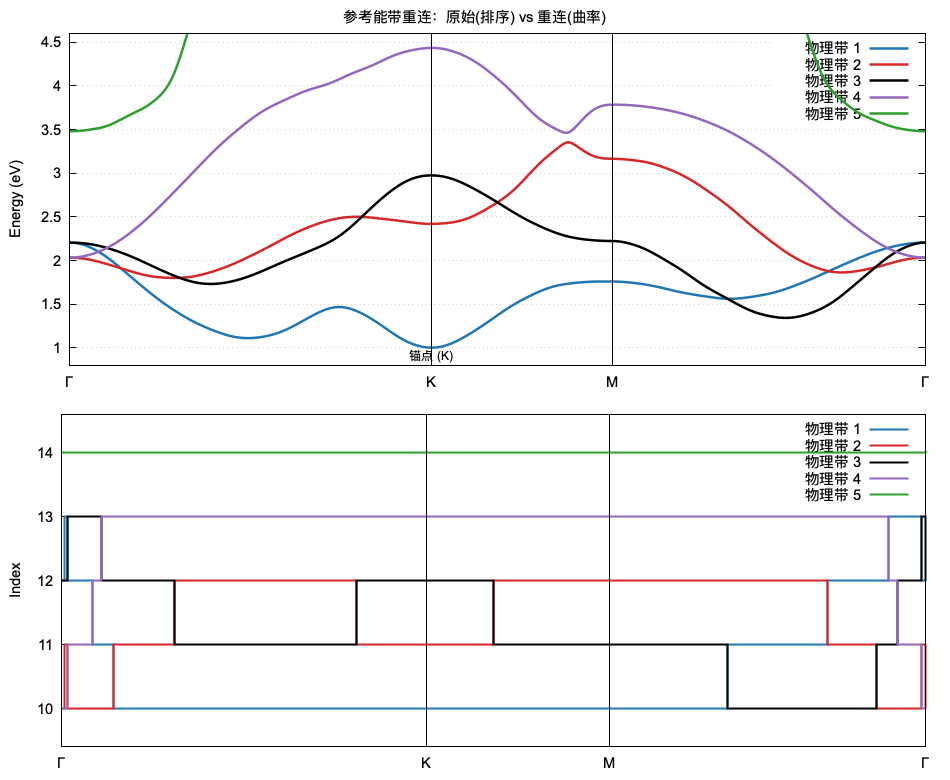
\includegraphics[width=\linewidth,height=0.62\textheight,keepaspectratio]{img/GW/reconnect.png}
    \end{column}
  \end{columns}
\end{frame}

%---------------------------------------------------------------------
\begin{frame}{拟合结果}
  \begin{columns}[T]
    \begin{column}{0.50\textwidth}
      \begin{itemize}
        \item 均方根偏差 $0.0334\,\mathrm{eV}$，初值是 $0.5531\,\mathrm{eV}$。
        \item 分带：价带 $0.0356$、第一导带 $0.0385$、第二导带 $0.0242\,\mathrm{eV}$。
        \item $K$ 点带隙 $2.6548\,\mathrm{eV}$，GW 参考 $2.6416\,\mathrm{eV}$，相差 $13\,\mathrm{meV}$。
        \item 这 13 meV 会整体平移到后面所有激子能级上。
      \end{itemize}
    \end{column}
    \begin{column}{0.48\textwidth}
      \centering
      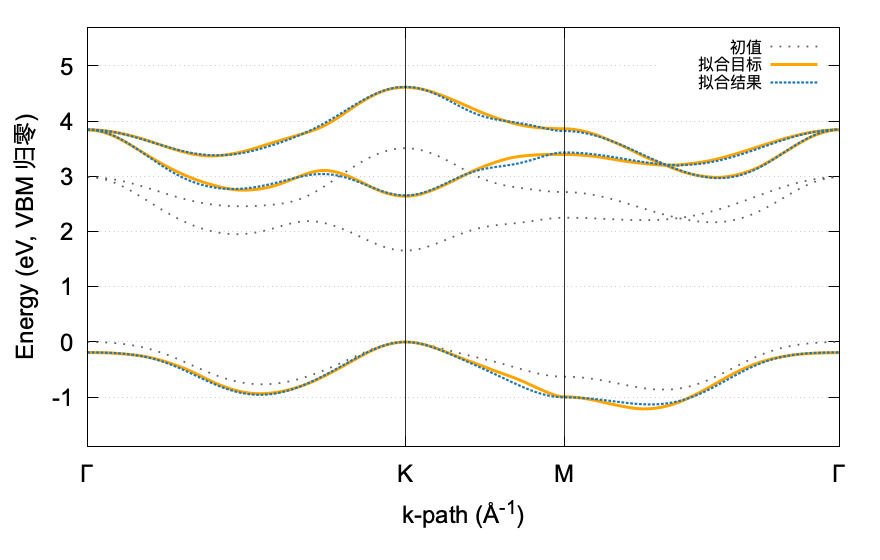
\includegraphics[width=\linewidth]{fig_fit.png}\\
      \scriptsize 灰点线为初值，橙线为 GW 参考，蓝虚线为拟合结果
    \end{column}
  \end{columns}
\end{frame}

%---------------------------------------------------------------------
\begin{frame}{模型：对上一阶段的一点修正}
  \begin{columns}[T]
    \begin{column}{0.54\textwidth}
      上个阶段我在画图的过程中没有注意能带相交的问题

      不过由于上个阶段拿到的参考数据只有在最后画图的时候有用，所以对模型的结果也没什么影响，只会影响画出来的图片的正确性

      所以也把上个阶段的结果图修正一下
    \end{column}
    \begin{column}{0.44\textwidth}
      \centering
      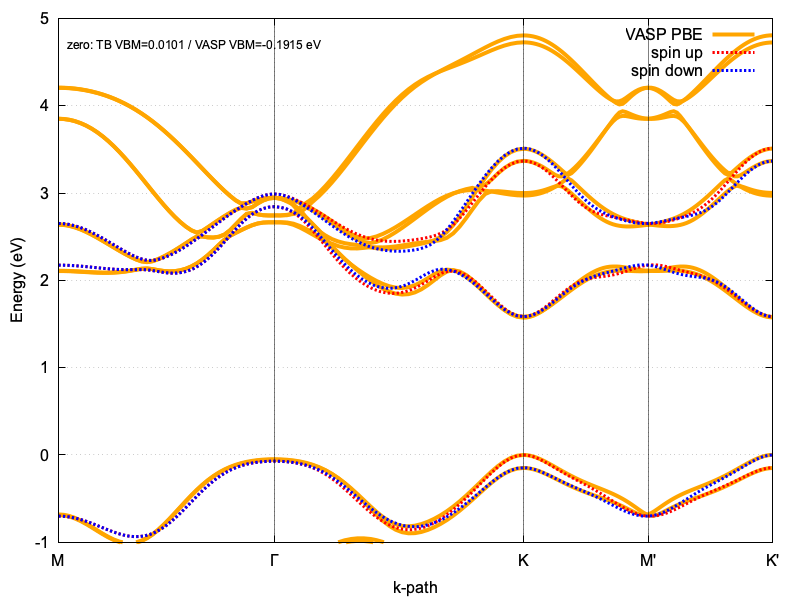
\includegraphics[height=0.50\textheight,keepaspectratio]{img/TB-reconnected/NN-NNN-TNN-SOC-SPIN.png}\\
      \scriptsize 上一阶段的能带（重新拼接后）
    \end{column}
  \end{columns}
\end{frame}

%---------------------------------------------------------------------
\begin{frame}{一点对比}
  \begin{columns}[T]
    \begin{column}{0.5\textwidth}
      \centering
      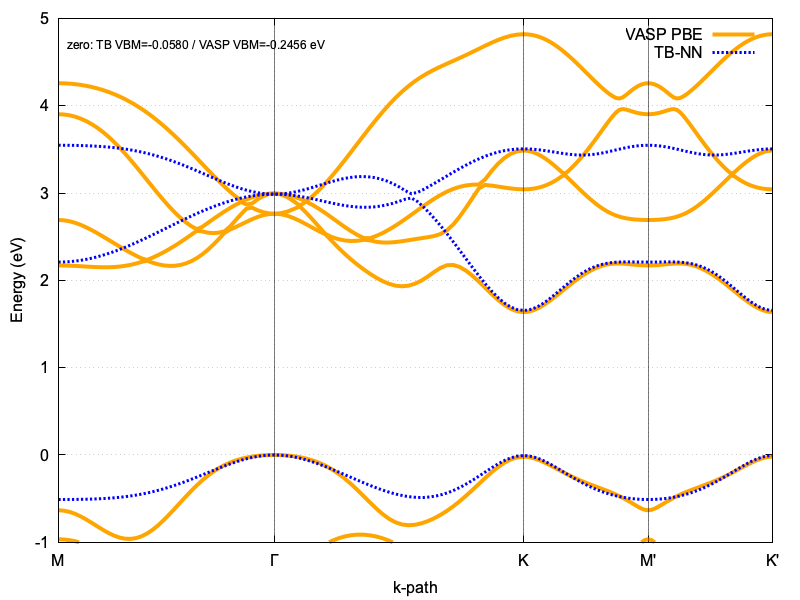
\includegraphics[height=0.50\textheight,keepaspectratio]{img/TB/NN.png}\\
      \scriptsize 上一阶段的能带（重新拼接前）
    \end{column}
    \begin{column}{0.5\textwidth}
      \centering
      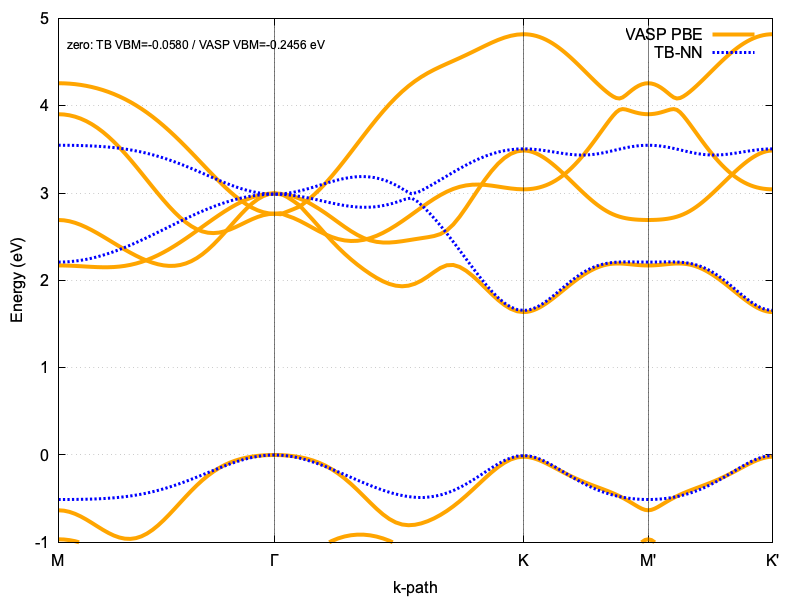
\includegraphics[height=0.50\textheight,keepaspectratio]{img/TB-reconnected/NN.png}\\
      \scriptsize 上一阶段的能带（重新拼接后）
    \end{column}
  \end{columns}
\end{frame}

%---------------------------------------------------------------------
\begin{frame}{一点对比}
  \begin{columns}[T]
    \begin{column}{0.5\textwidth}
      \centering
      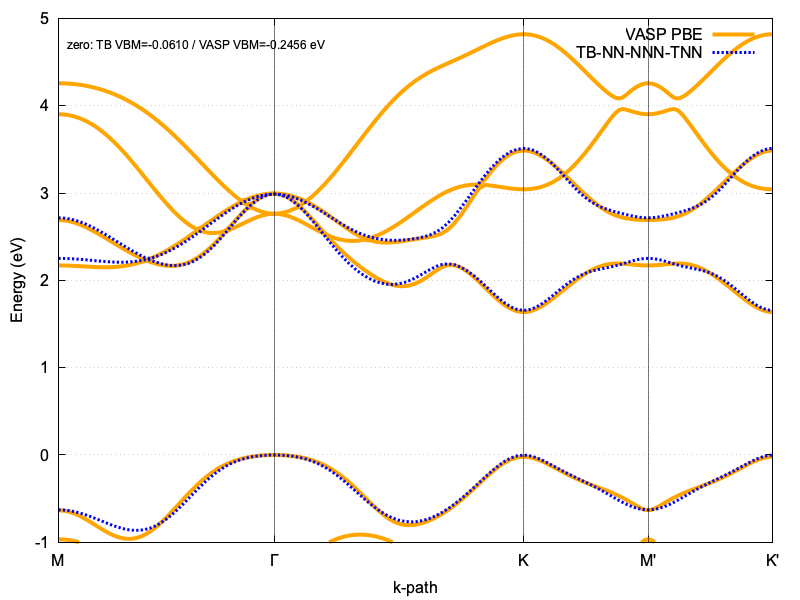
\includegraphics[height=0.50\textheight,keepaspectratio]{img/TB/NN-NNN-TNN.png}\\
      \scriptsize 上一阶段的能带（重新拼接前）
    \end{column}
    \begin{column}{0.5\textwidth}
      \centering
      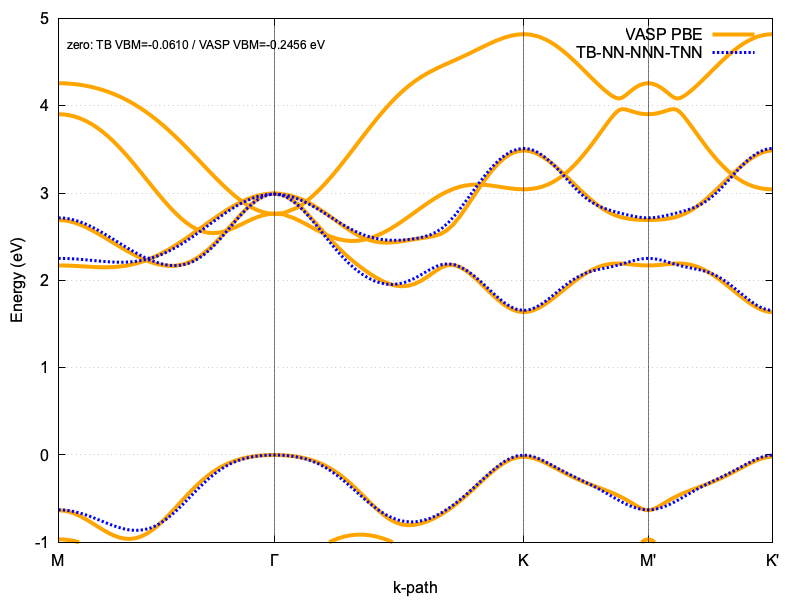
\includegraphics[height=0.50\textheight,keepaspectratio]{img/TB-reconnected/NN-NNN-TNN.png}\\
      \scriptsize 上一阶段的能带（重新拼接后）
    \end{column}
  \end{columns}
\end{frame}

%---------------------------------------------------------------------
\begin{frame}{一点对比}
  \begin{columns}[T]
    \begin{column}{0.5\textwidth}
      \centering
      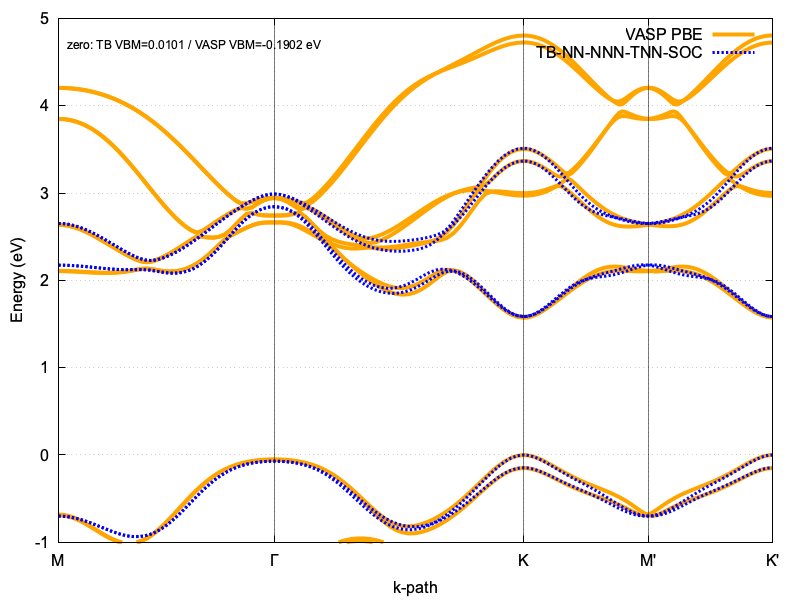
\includegraphics[height=0.50\textheight,keepaspectratio]{img/TB/NN-NNN-TNN-SOC.png}\\
      \scriptsize 上一阶段的能带（重新拼接前）
    \end{column}
    \begin{column}{0.5\textwidth}
      \centering
      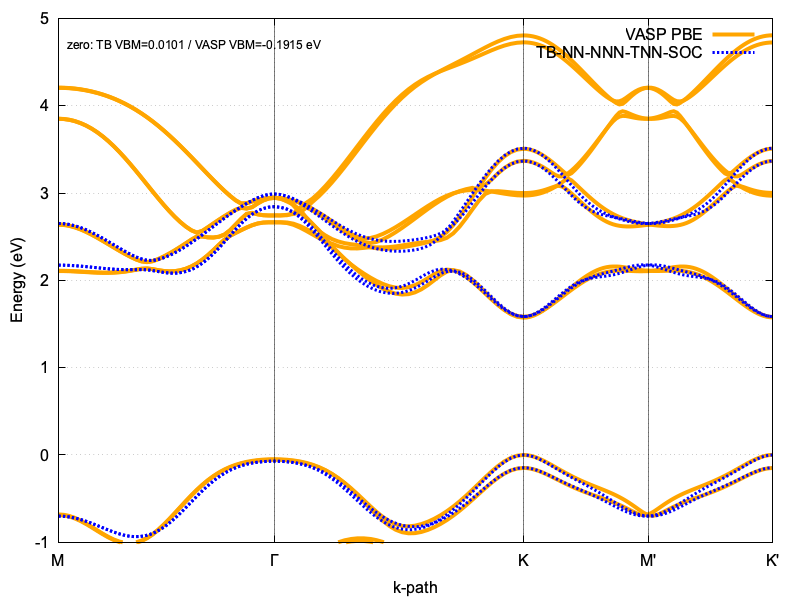
\includegraphics[height=0.50\textheight,keepaspectratio]{img/TB-reconnected/NN-NNN-TNN-SOC.png}\\
      \scriptsize 上一阶段的能带（重新拼接后）
    \end{column}
  \end{columns}
\end{frame}

%---------------------------------------------------------------------
\begin{frame}{一点对比}
  \begin{columns}[T]
    \begin{column}{0.5\textwidth}
      \centering
      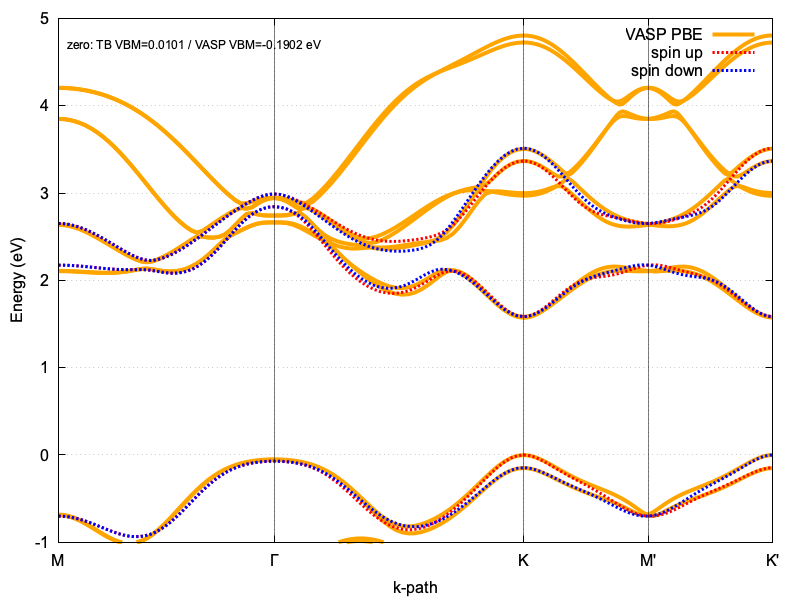
\includegraphics[height=0.50\textheight,keepaspectratio]{img/TB/NN-NNN-TNN-SOC-SPIN.png}\\
      \scriptsize 上一阶段的能带（重新拼接前）
    \end{column}
    \begin{column}{0.5\textwidth}
      \centering
      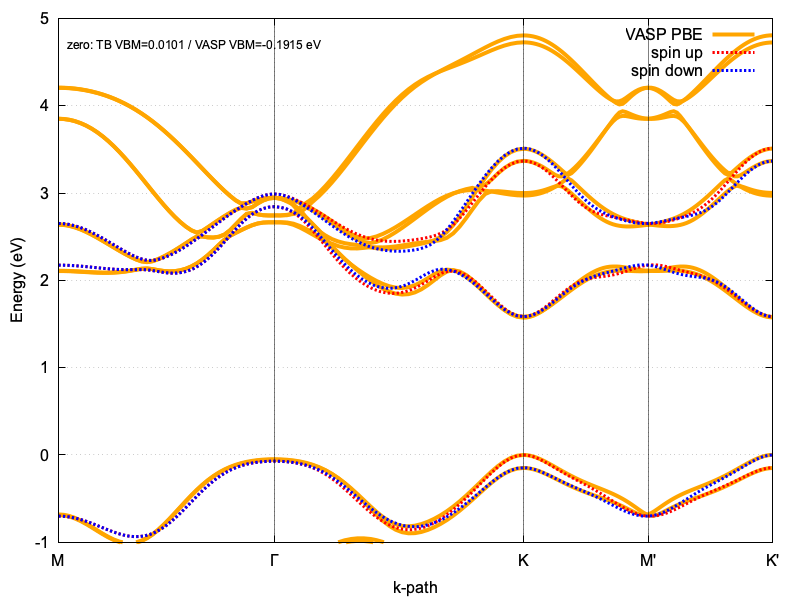
\includegraphics[height=0.50\textheight,keepaspectratio]{img/TB-reconnected/NN-NNN-TNN-SOC-SPIN.png}\\
      \scriptsize 上一阶段的能带（重新拼接后）
    \end{column}
  \end{columns}
\end{frame}

%---------------------------------------------------------------------
\begin{frame}{算法的局限性}
  这套算法在处理自旋导致的能带劈裂时表现一般。
  原因主要在于劈裂的能带在一些位置会简并，这就导致最小曲率的排序时存在
  一定的随机性：\par
  \vspace{1mm}
  $\Gamma$、K、M'、K' 处 Up 与 Dn 两支恰好重合，拼接会在这些点重新挑边，
  之后的归属可能整体对调。
  \begin{center}
  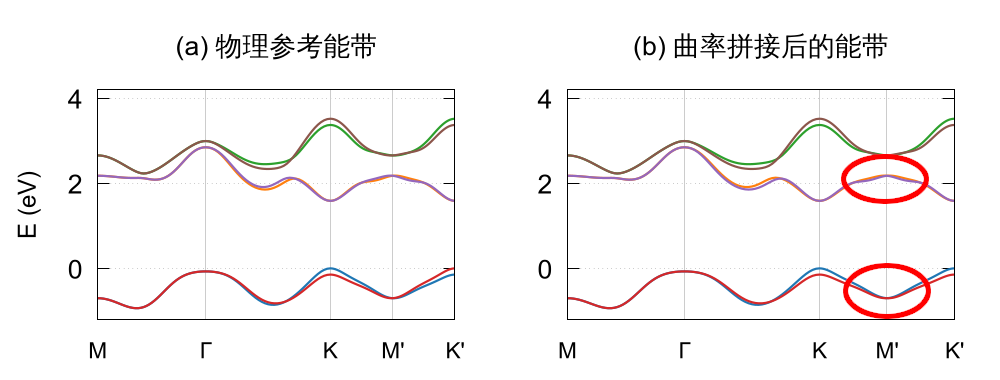
\includegraphics[width=0.96\textwidth]{soc_stitch_cmp.png}
  \end{center}
\end{frame}

%---------------------------------------------------------------------
\begin{frame}[plain]
  \centering
  {\color{accent}\Huge\bfseries 第二部分}\\[7mm]
  {\Large 一些公式的计算}\\[4mm]
  {\small E. Ridolfi, C. H. Lewenkopf, V. M. Pereira,
  \emph{Phys. Rev. B} \textbf{97}, 205409 (2018)}
\end{frame}

%---------------------------------------------------------------------
\begin{frame}{目标 2：把式 (6) 的核算出来}
  \framesubtitle{论文式 (6)--(10)、(17)}
  \small
  \begin{columns}[T]
    \begin{column}{0.52\textwidth}
      \textbf{已知}
      \begin{enumerate}
        \item 紧束缚哈密顿量 $H(\kk)$
        \item 每个 $\kk$ 点的本征值 $\eps_{n\kk}$ 与本征矢 $C^{n}_{\alpha\kk}$
        \item 屏蔽库仑势 $u(q)$ 与参数 $r_0$、$\eps_d$
      \end{enumerate}
      \textbf{求}：对全部 $\kk,\kq$ 与 $c,c',v,v'$
      \begin{equation*}
        W^{(d)}_{cv\kk,c'v'\kq}=u(\kk-\kq)\,I^{*}_{c'\kq,c\kk}\,I_{v'\kq,v\kk}
      \end{equation*}
      \textbf{产出}：$N_{\mathrm{tot}}=N_k^2N_cN_v$ 维方阵
    \end{column}
    \begin{column}{0.44\textwidth}
      \small 这个核是论文式 (5) 左边的核：
      \resizebox{\linewidth}{!}{$\displaystyle
        E_{cv\kk}A^{M}_{cv\kk}
        +\frac{1}{V}\sum_{c'v'\kq}W_{cv\kk,c'v'\kq}A^{M}_{c'v'\kq}
        =E_{M}A^{M}_{cv\kk}$}
      \scriptsize 其中 $|M\rangle=\sum_{cv\kk}A^{M}_{cv\kk}|v\kk\to c\kk\rangle$。
      怎么解式 (5) 属于目标 3
    \end{column}
  \end{columns}
\end{frame}


%---------------------------------------------------------------------
\begin{frame}{符号对照表}
  \framesubtitle{最后一列是本课题模型的实际取值}
  \centering
  \footnotesize
  \begin{tabular}{@{}lll@{}}
    \toprule
    符号 & 含义 & 本课题取值\\
    \midrule
    $\kk,\kq$ & 布里渊区里的两个 $k$ 点 & 均匀网格，共 $N_k^2$ 个\\
    $c,c'$ & 导带编号 & 2 条\\
    $v,v'$ & 价带编号 & 1 条\\
    $\alpha$ & 轨道编号 & 6 个（3 个 $d$ 轨道 $\times$ 2 个自旋）\\
    $C^{n}_{\alpha\kk}$ & 第 $n$ 条带在轨道 $\alpha$ 上的分量 & 复数，$|C|\le1$\\
    $\eps_{n\kk}$ & 第 $n$ 条带的能量 & eV\\
    $u(q)$ & 屏蔽库仑势 & eV$\cdot$\AA$^2$\\
    $I$ & 两条 Bloch 态的轨道交叠 & 无量纲，$|I|\le1$\\
    $N_k$ & 每个方向的 $k$ 点数 & 文献取 60\\
    $A_c$ & 原胞面积 $\sqrt3a^2/2$ & $8.65$~\AA$^2$\\
    $V$ & 晶体总面积 $A_cN_k^2$ & $N_k=60$ 时 $3.1\times10^4$~\AA$^2$\\
    \bottomrule
  \end{tabular}
\end{frame}


%---------------------------------------------------------------------
\begin{frame}{第一步：解 $H(\kk)$，得到本征值和本征矢}
  \framesubtitle{论文式 (1)--(2)}
  \begin{equation*}
    H(\kk)\,\mathbf u_{n\kk}=\eps_{n\kk}\,\mathbf u_{n\kk},
    \qquad
    \mathbf u_{n\kk}=\big(C^{n}_{1\kk},C^{n}_{2\kk},\dots,C^{n}_{\alpha\kk}\big)^{T}
  \end{equation*}
  \begin{itemize}
    \item $\mathbf u_{n\kk}$ 是列向量，长度等于轨道数，本课题是 6。
    \item 把 6 个本征问题都解出来，得到 6 个 $\eps_{n\kk}$ 和 6 个长度为 6 的列向量。
    \item $6\times6$ 矩阵不方便手算，交给数值对角化。
    \item 解出来的本征矢必须归一化，否则后面算出的交叠积分会整体偏大或偏小。
  \end{itemize}
\end{frame}


%---------------------------------------------------------------------
\begin{frame}{第二步：把本征矢的相位定死}
  \framesubtitle{论文式 (7) 之后}
  \begin{itemize}
    \item 本征矢不是唯一的：$\mathbf u$ 是本征矢，$e^{\mathrm{i}\varphi}\mathbf u$ 也是，
          因为 $H(e^{\mathrm{i}\varphi}\mathbf u)=e^{\mathrm{i}\varphi}\eps\mathbf u$。
    \item 这个相位任意性必须先定下来，否则每次算出的交叠积分都不同。
    \item 做法：把每条带在轨道上的分量加起来
  \end{itemize}
  \begin{equation*}
    S_{n\kk}=\sum_{\alpha}C^{n}_{\alpha\kk},
    \qquad
    C^{n}_{\alpha\kk}\;\longrightarrow\;C^{n}_{\alpha\kk}\,e^{-\mathrm{i}\arg S_{n\kk}},
    \qquad\text{从而}\qquad
    \sum_{\alpha}C^{n}_{\alpha\kk}\in\mathbb{R}
  \end{equation*}
  \begin{itemize}
    \item 退化情形：若某条带的 $S_{n\kk}=0$，辐角无法定义，这个办法失效。
          这时改用平行移动，让相邻 $k$ 点上的内积为正实数，逐点定相位。
  \end{itemize}
\end{frame}


%---------------------------------------------------------------------
\begin{frame}{第三步：算轨道交叠积分 $I$}
  \framesubtitle{论文式 (7)}
  \begin{equation*}
    I_{a\kq,b\kk}=\sum_{\alpha}C^{a*}_{\alpha\kq}\,C^{b}_{\alpha\kk}
  \end{equation*}
  \begin{itemize}
    \item 就是两个长度为 6 的复向量的内积：$\kq$ 点第 $a$ 条带的向量与 $\kk$ 点第 $b$ 条带的向量，
          逐分量相乘（第一个取复共轭）再相加。
    \item $I=1$ 表示两个态完全一样，$I=0$ 表示正交，一般介于两者之间。
  \end{itemize}
  \vspace{2mm}
  \begin{block}{三条可以拿来验证的性质}
    \begin{enumerate}
      \item 同一个 $k$ 点上同一条带：$I_{a\kk,a\kk}=\sum_\alpha|C^{a}_{\alpha\kk}|^2=1$（归一化）
      \item 同一个 $k$ 点上不同能带：$I_{a\kk,b\kk}=0$（本征矢互相正交）
      \item 交换上下指标取复共轭：$I_{a\kq,b\kk}=I^{*}_{b\kk,a\kq}$
    \end{enumerate}
  \end{block}
\end{frame}


%---------------------------------------------------------------------
\begin{frame}{第四步：算屏蔽库仑势 $u(q)$}
  \framesubtitle{论文式 (8)--(10)}
  \begin{equation*}
    u(q)=-\frac{e^2}{2\eps_0\eps_d\,q\,(1+r_0q)},
    \qquad
    \eps_d=\frac{\eps_1+\eps_3}{2},
    \qquad
    r_0=\frac{2\eps_2^2-\eps_1^2-\eps_3^2}{2\eps_2(\eps_1+\eps_3)}\,d
  \end{equation*}
  \begin{itemize}
    \item $q$ 是两个 $k$ 点之差的长度
          $q=|\kk-\kq|=\sqrt{(k_x-k'_x)^2+(k_y-k'_y)^2}$，不是一维的数。
    \item $u$ 只依赖这个长度，与方向无关，所以可以预先按 $q$ 做成表，需要时查表。
    \item 两个区域：$r_0q\ll1$ 时 $u\propto1/q$，对应实空间长程 $1/r$；
          $r_0q\gg1$ 时 $u\propto1/q^2$。分界在 $q\approx1/r_0=0.074$~\AA$^{-1}$。
  \end{itemize}
\end{frame}


%---------------------------------------------------------------------
\begin{frame}{第五步：把三个数乘起来}
  \framesubtitle{论文式 (6)}
  \begin{equation*}
    W^{(d)}_{cv\kk,c'v'\kq}
    =\underbrace{u(\kk-\kq)}_{\text{实数}}\cdot
    \underbrace{I^{*}_{c'\kq,c\kk}}_{\text{复数}}\cdot
    \underbrace{I_{v'\kq,v\kk}}_{\text{复数}}
  \end{equation*}
  \begin{itemize}
    \item 到这一步三样东西都有了，按式 (6) 直接相乘即可。
    \item 乘积一般仍是复数，因为两个 $I$ 来自不同的带。
    \item 注意式 (5) 里还有一个 $1/V$，矩阵里存的是 $W^{(d)}/V$，量级才和激子能量对得上。
  \end{itemize}
\end{frame}


%---------------------------------------------------------------------
\begin{frame}{第六步：$\kk=\kq$ 的对角元要单独处理}
  \framesubtitle{论文式 (17)}
  \begin{itemize}
    \item $\kq=\kk$ 时 $q=0$，$u$ 在 $q=0$ 处分母为零。
    \item 处理办法是换成 $q=0$ 附近小区域上的平均值：
  \end{itemize}
  \resizebox{0.95\linewidth}{!}{$\displaystyle
    u(\qq\approx0)\;\longrightarrow\;\frac{1}{\Delta q}\int_{\Delta q}u(\qq)\,\mathrm d\qq
    \approx-\frac{e^2aN_k}{4\pi\eps_0\eps_d}\left[\alpha_1+\alpha_2\frac{2\pi r_0}{aN_k}
    +\alpha_3\left(\frac{2\pi r_0}{aN_k}\right)^2\right]$}
  \vspace{2mm}
  \begin{itemize}
    \item $\Delta q$ 是每个 $k$ 点在倒空间里代表的面积；$\alpha_{1,2,3}$ 由小区域形状和展开阶数决定。
    \item 展开参数 $\dfrac{2\pi r_0}{aN_k}=\dfrac{26.9}{N_k}$，$N_k=60$ 时是 $0.45$，不算小，
          所以 $\alpha_2,\alpha_3$ 不能随便丢。只留 $\alpha_1$ 时收敛明显慢（论文图 2）。
  \end{itemize}
\end{frame}


%---------------------------------------------------------------------
\begin{frame}{第七步：把矩阵元排成矩阵}
  \framesubtitle{论文式 (5)、(6)}
  \begin{itemize}
    \item 行列都用三元组 $(\kk,c,v)$ 编号，$k$ 点的线性编号记作 $i_k$：
          \[
          \text{行号}=i_k\,(N_cN_v)+i_c\,N_v+i_v
          \]
    \item 排好之后式 (5) 就是标准本征值问题
  \end{itemize}
  \resizebox{0.95\linewidth}{!}{$\displaystyle
    \mathcal{H}_{(c\kk),(c'\kq)}
    =\delta_{cc'}\delta_{\kk\kq}E_{cv\kk}
    +\frac{1}{A_cN_k^2}\,u(\kk-\kq)\,I^{*}_{c'\kq,c\kk}\,I_{v'\kq,v\kk}$}
  \vspace{2mm}
  \begin{itemize}
    \item 厄米性：由 $I_{a\kq,b\kk}=I^{*}_{b\kk,a\kq}$ 与 $u(-\qq)=u(\qq)$，交换行列并取复共轭得到同一个值。
    \item 厄米很重要：它保证解出来的 $E_M$ 是实数。
  \end{itemize}
\end{frame}


%---------------------------------------------------------------------
\begin{frame}{检查答案}
  \framesubtitle{四条验算}
  \begin{enumerate}
    \item \textbf{归一化检查。} 对每条带、每个 $k$ 点算 $I_{a\kk,a\kk}$，应当等于 1；
          偏离 1 的量级就是对角化的精度。
    \item \textbf{相位检查。} 固定相位前后 $I_{n\kq,n\kk}$ 的相位不应跳变，
          相邻 $k$ 点上模应当接近 1 并逐渐下降。相位随机跳说明第二步没做对。
    \item \textbf{厄米检查。} 抽若干对矩阵元验 $\mathcal{H}_{ij}=\mathcal{H}^{*}_{ji}$；
          不成立通常是行号编错，或 $I$ 的复共轭取反了。
    \item \textbf{收敛检查。} 把 $N_k$ 从 30 加到 60，看最低激子能级是否单调趋于稳定值。
          正则化方案选择不当会让它收敛很慢或来回摆。
  \end{enumerate}
\end{frame}


%---------------------------------------------------------------------
\begin{frame}{对比}
  \centering
  \small
  \begin{tabular}{@{}lll@{}}
    \toprule
     & 文献 & 我们 \\
    \midrule
    基组 & 11 个原子轨道 & 3 个 $d$ 轨道 \\
    拟合参数 & 14 个 & 19 个 \\
    拟合目标 & 他们自己的 GW 能带 & 我们的 GW 能带（Wannier90 插值）\\
    $K$ 点带隙 & $2.115\,\mathrm{eV}$ & $2.6548\,\mathrm{eV}$ \\
    能量范围 & 到紫外，含 C 峰 & 带边 A、B 激子 \\
    \bottomrule
  \end{tabular}
  \vspace{5mm}
  \begin{itemize}
    \item 同一个思路的两个规模：轨道少、参数少换来速度，代价是高能结构描述不了。
    \item 可以直接借鉴的是屏蔽势的取法与 $r_0$（式 8--10）、BSE 核与规范固定（式 6、7），
      以及 $q\to0$ 奇异性的正则化（式 17）。
  \end{itemize}
\end{frame}

%---------------------------------------------------------------------
\begin{frame}{\Large 参考文献：}
  \small 
  E. Ridolfi, C. H. Lewenkopf, V. M. Pereira, \emph{Phys. Rev. B} \textbf{97}, 205409 (2018). DOI: 10.1103/PhysRevB.97.205409\\
\end{frame}

%---------------------------------------------------------------------
\begin{frame}
  \centering
  {\Huge 感谢聆听}
\end{frame}

\end{document}
